
\section{Design}

\subsection{Overall Concept}

The design goals for the proposed labview architecture are as follows:

\begin{enumerate}
  \item{Intuitive to new users}
  \item{Expandable}
  \item{Improved fault tolerance}
  \item{Flexibility to accommodate hardware configuration changes}
  \item{Improved data quality \& collection uptime}
  \item{Algoritm isolation for testing and run-time stability}
\end{enumerate}

To accomplish these goals, the following concept is proposed. Small individual programs are written to control conceptually seperate processes which interact with the WV DIAL hardware in various ways. These small programs can run in parallel with proper synchronization and communication. A main sub-function is used to call collections of various individual programs and opens the necessary individual program automatically. These sub-functions are all called by the main function based on user input for what the software should do***specify here***. The operational setups that are called by the main function are: ***fill in list***

\begin{enumerate}
	\item{Warm up sub-function that brings all hardware to operational status. This includes things like warming the lasers and warming the etalons, which needs to be done before high quality data can be taken.}
	\item{Main operations sub-function that performs all the mission critical hardware communication during data collection.}***split this up into pieces, don't have one master subfunction***
	\item{Testing sub-functions to check operational status of individual hardware pieces such as the laser locking or the MCS operation or the weather station.}
\end{enumerate}

This creates a 3 tiered structure: 1) Main function that opens sub-functions, 2) Sub-functions that organize and manage individual controls, and 3) Individual controls that actually set and control the state of each individual hardware piece. This overall structure accomplishes the main goals in a number of ways. There is a natural hierarchy that is predefined. New users unfamiliar with the operation of WV DIAL do not need to know how to control each piece individually but rather are guided through operation via button clicks. Testing new hardware does not require complete integration with an all in one solution like is currently available. The system is fault tolerant because all tasks are separated. If one task fails, others are not waiting on that task. Finally, knowledge of the hardware configuration is only needed at the higher levels, main function and sub-functions, and can be more easily defined than a single all in one program. 

\subsection{Individual Element Controls}
The proposed software update parses the main hardware control function into many small functions. Having multiple small sub-functions running facilitates the new software design goals in a number of key ways. First, there is expandability because new VIs can be easily added that do no affect the old VIs. They do affect the methods in which the old VIs communicate however and require standardized communication practices. Second, fault tolerance is accomplished by splitting mission critical elements from non-critical elements. Third, hardware configurations are simple to accommodate; they only require the main function to know what is currently plugged in and where. Finally, testing of hardware can be done more easily and with fewer confounding variables as each piece of code does not rely on others to be running to be tested. A list of elements that would have their own controls are:

\begin{enumerate}
	\item{MCS setup, configuration, and data saving}
	\item{Weather station acquisition and data saving}
	\item{Laser locking and housekeeping data saving}
	\item{Receiver etalon temperature control and data saving}
	\item{Data visualization}
		\begin{enumerate}
			\item{Alignment profiles: raw data and background subtracted data}
			\item{Weather Station and laser housekeeping}
			\item{Retrieved profiles: optical depth, number density, absolute humidity, ... }
			\item{Retrieved contour plots: normalized relative backscatter, number density, backscatter coefficient,~...}
		\end{enumerate}
	\item{Hardware Testing Routines}
		\begin{enumerate}
			\item{Individual switch control: this has been used in the past to check on the status and wavelengths of the lasers as the lasers are being aligned or to force only a single laser into the TSOA or to test isolation and spectral purity}
			\item{Receiver wavelength scan: used to map the transmission of the receiver as a function of wavelength}
			\item{Receiver temperature scan: used to locate the transmission band of the etalon}
		\end{enumerate}
\end{enumerate}

\subsubsection{Back Panel Design}\label{Sec:BPDesign}

A template was made to standardize all labview control for WV DIAL. The back panel of the template is meant to be a template as well as the front. The idea is to use a queue to execute commands using a single function. This allows for an intentional bottleneck of execution such that user and automatically generated commands can not be executed out of order and there are a minimum of changes that need to be made to accommodate new hardware. The automatically generated and user generated commands are in the form of a string that is delimitated by a ``\_". The main loop cases are:
\begin{enumerate}
	\item{Configure}
	\begin{enumerate}
		\item{Reads default state out of the configure file}
		\item{Sets the value of all available controls per the configure file}
		\item{Sets the function visibility based on control settings like RunAsChild and permissions settings}
		\item{Performs logging of any known or anomalous states}
	\end{enumerate}
	\item{Initialize}
	\begin{enumerate}
		\item{Communicate the initial state of the labview controls to the hardware or vice versa as appropriate}
		\item{Create needed file folders for data saving}
		\item{Performs logging of any known or anomalous states}
	\end{enumerate}
	\item{Idle}
	\begin{enumerate}
		\item{Performs baseline commands needed to keep program running}
		\item{Waits for user commands to change the state of the system}
		\item{Performs all commands and communication with the global variables}
		\item{Allows for any data visualization}
		\item{Performs logging of any known or anomalous states}
	\end{enumerate}
	\item{Error Handler}
	\begin{enumerate}
		\item{Records all errors in an error log for debugging}
		\item{Attempts recovery procedure if the error is recognized}
		\item{Alerts the user if error are time sensitive or mission critical}
		\item{Performs logging of any known or anomalous states}
	\end{enumerate}
	\item{Commanded Exit}
	\begin{enumerate}
		\item{Performs necessary steps to shutdown hardware that are specific to being told to shut down (only accessible in RunAsChild mode)}
		\item{Performs logging of any known or anomalous states}
	\end{enumerate}
	\item{Exit}
	\begin{enumerate}
		\item{Performs necessary steps to shutdown hardware that are general to RunAsChild or not}
		\item{Makes all hidden variables visible again for coding}
		\item{Performs logging of any known or anomalous states}
	\end{enumerate}
\end{enumerate}


\begin{figure}[!h]\centering
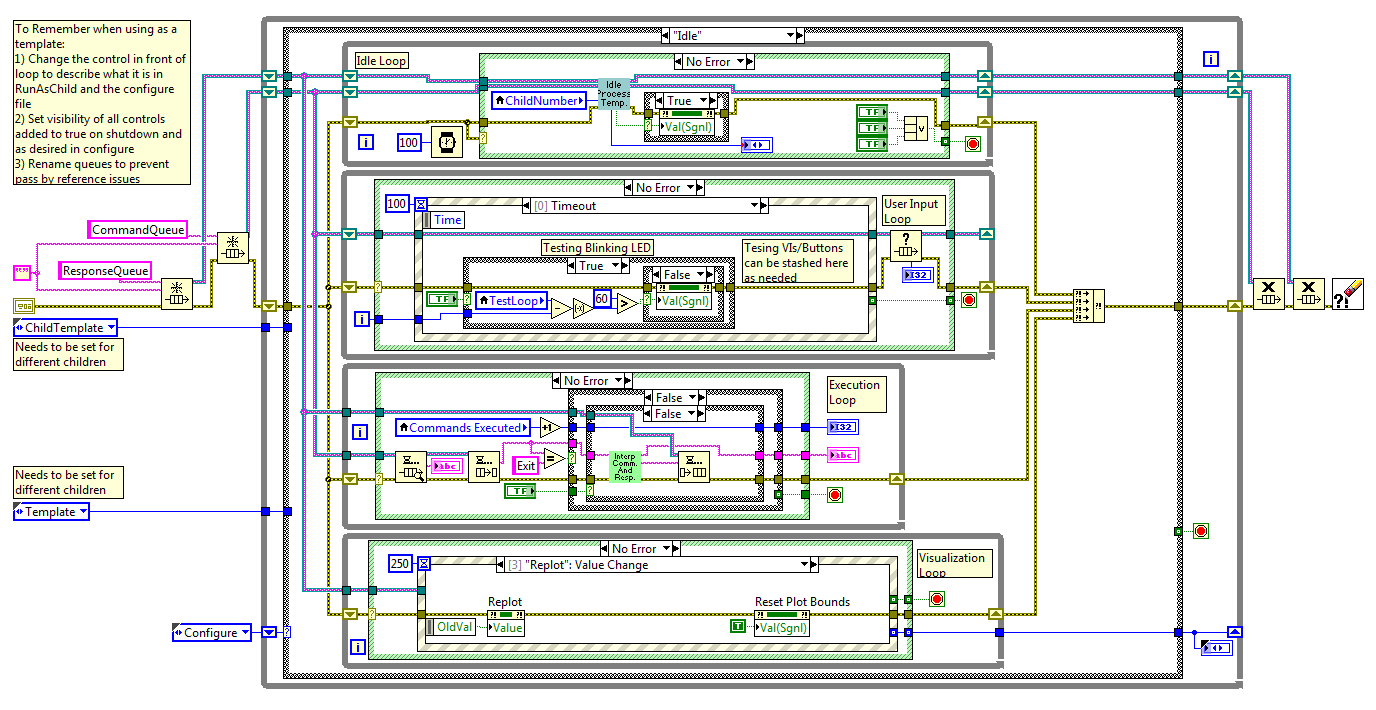
\includegraphics[height=3in]{Figures/MainVITemplateBackPanel.eps}
\caption{A picture of the idle loop stage of the VI template for the individual element control. In the idle loop, 3 while loops run. The top loop is waiting for user input or executing commands that are needed to maintain control of the hardware. The middle loop is waiting for user commands or idle commands and is executing them. Critically, this function is called in re-entrant execution mode as it is copied in all functions. The lowest loop is visualizing data as it is being recorded. The top loop should be filled with system specific commands relating to system specific controls.}\label{Fig:VITemplateBP}
\end{figure}


\subsubsection{Run as Stand Alone}

The multiple function concept requires one functional distinction. One concept is to run each piece manually, and another is to have a main function run each piece automatically, refered to as running in stand along mode or running as child, respectively.   

A template for the individual control elements is given in Figure \ref{Fig:VITemplate}. It is based on a queue structure in the back panel that allows both user commands and automatic commands to fill the queue that is then emptied by a single hardware function. There are 3 main boxes, the first is in the top left (labeled as ``Place Commands Here") for all of the user controls and everything the user needs to see. This will be different for each control. Within that box is a smaller box that would be the same for all controls that help locate the current status of the queue. The second box directly below would appear if the control were running as a stand alone but be hidden if the control were running as child. This really only needs to be in one place and is constant for all functions. The final box to the right is always hidden but is the storage place for all hidden variables that need to be defined but that the user does not need to see. 

\begin{figure}[!h]\centering
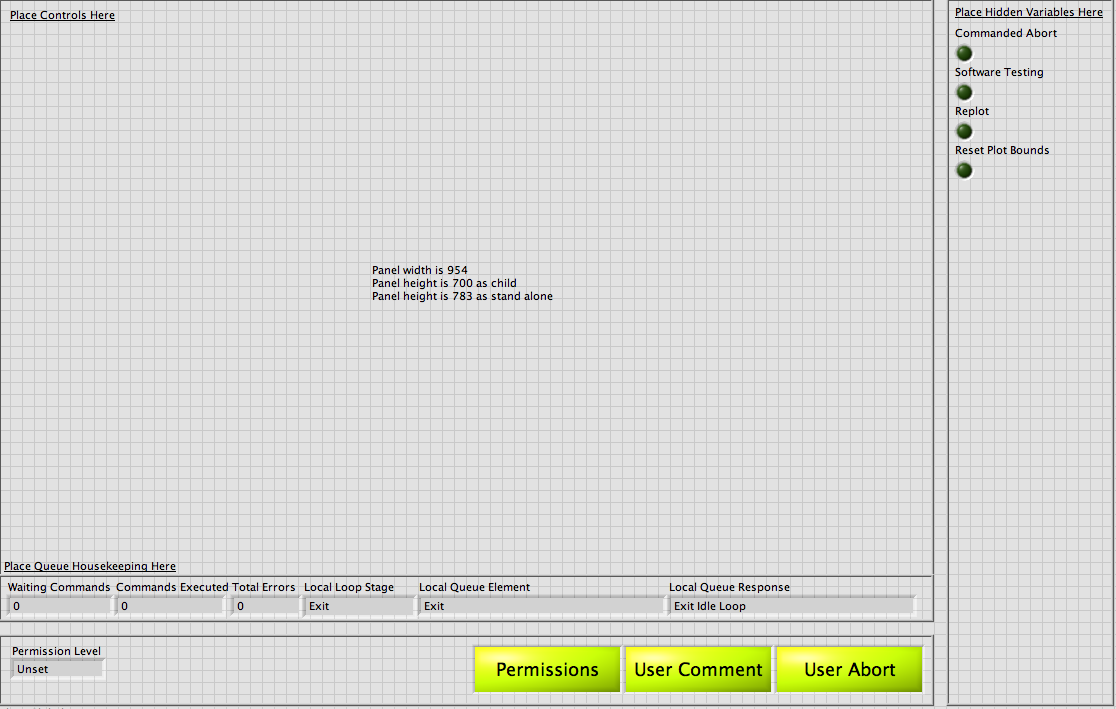
\includegraphics[height=3in]{Figures/MainVITemplate.eps}
\caption{The front panel of the main VI template. The software at runtime will hide the unnecessary controls and shrink the front panel window the the appropriate size indicated by the outer boxes. If the VI is run as a child (called from a higher VI) the Global Buttons disappear. }\label{Fig:VITemplate}
\end{figure}

This standardization is not critical for running all VIs as stand alone, however, the solution for running all the VIs as children in parallel does. 

\subsubsection{Run as Child}

For the case that these individual controls are to be run automatically in parallel, an organizational problem arises. Assuming the code running the individual controls as children knows what functions to open and in what order, it is still possible that a user accidentally closes one function or a mess of VIs appears. To solve this, all front panels of the VIs running are projected into a single container. The container itself has very little code running but is just there to contain all of the sub-VIs. This container is shown in Figure \ref{Fig:VIContainer}.

\begin{figure}[!h]\centering
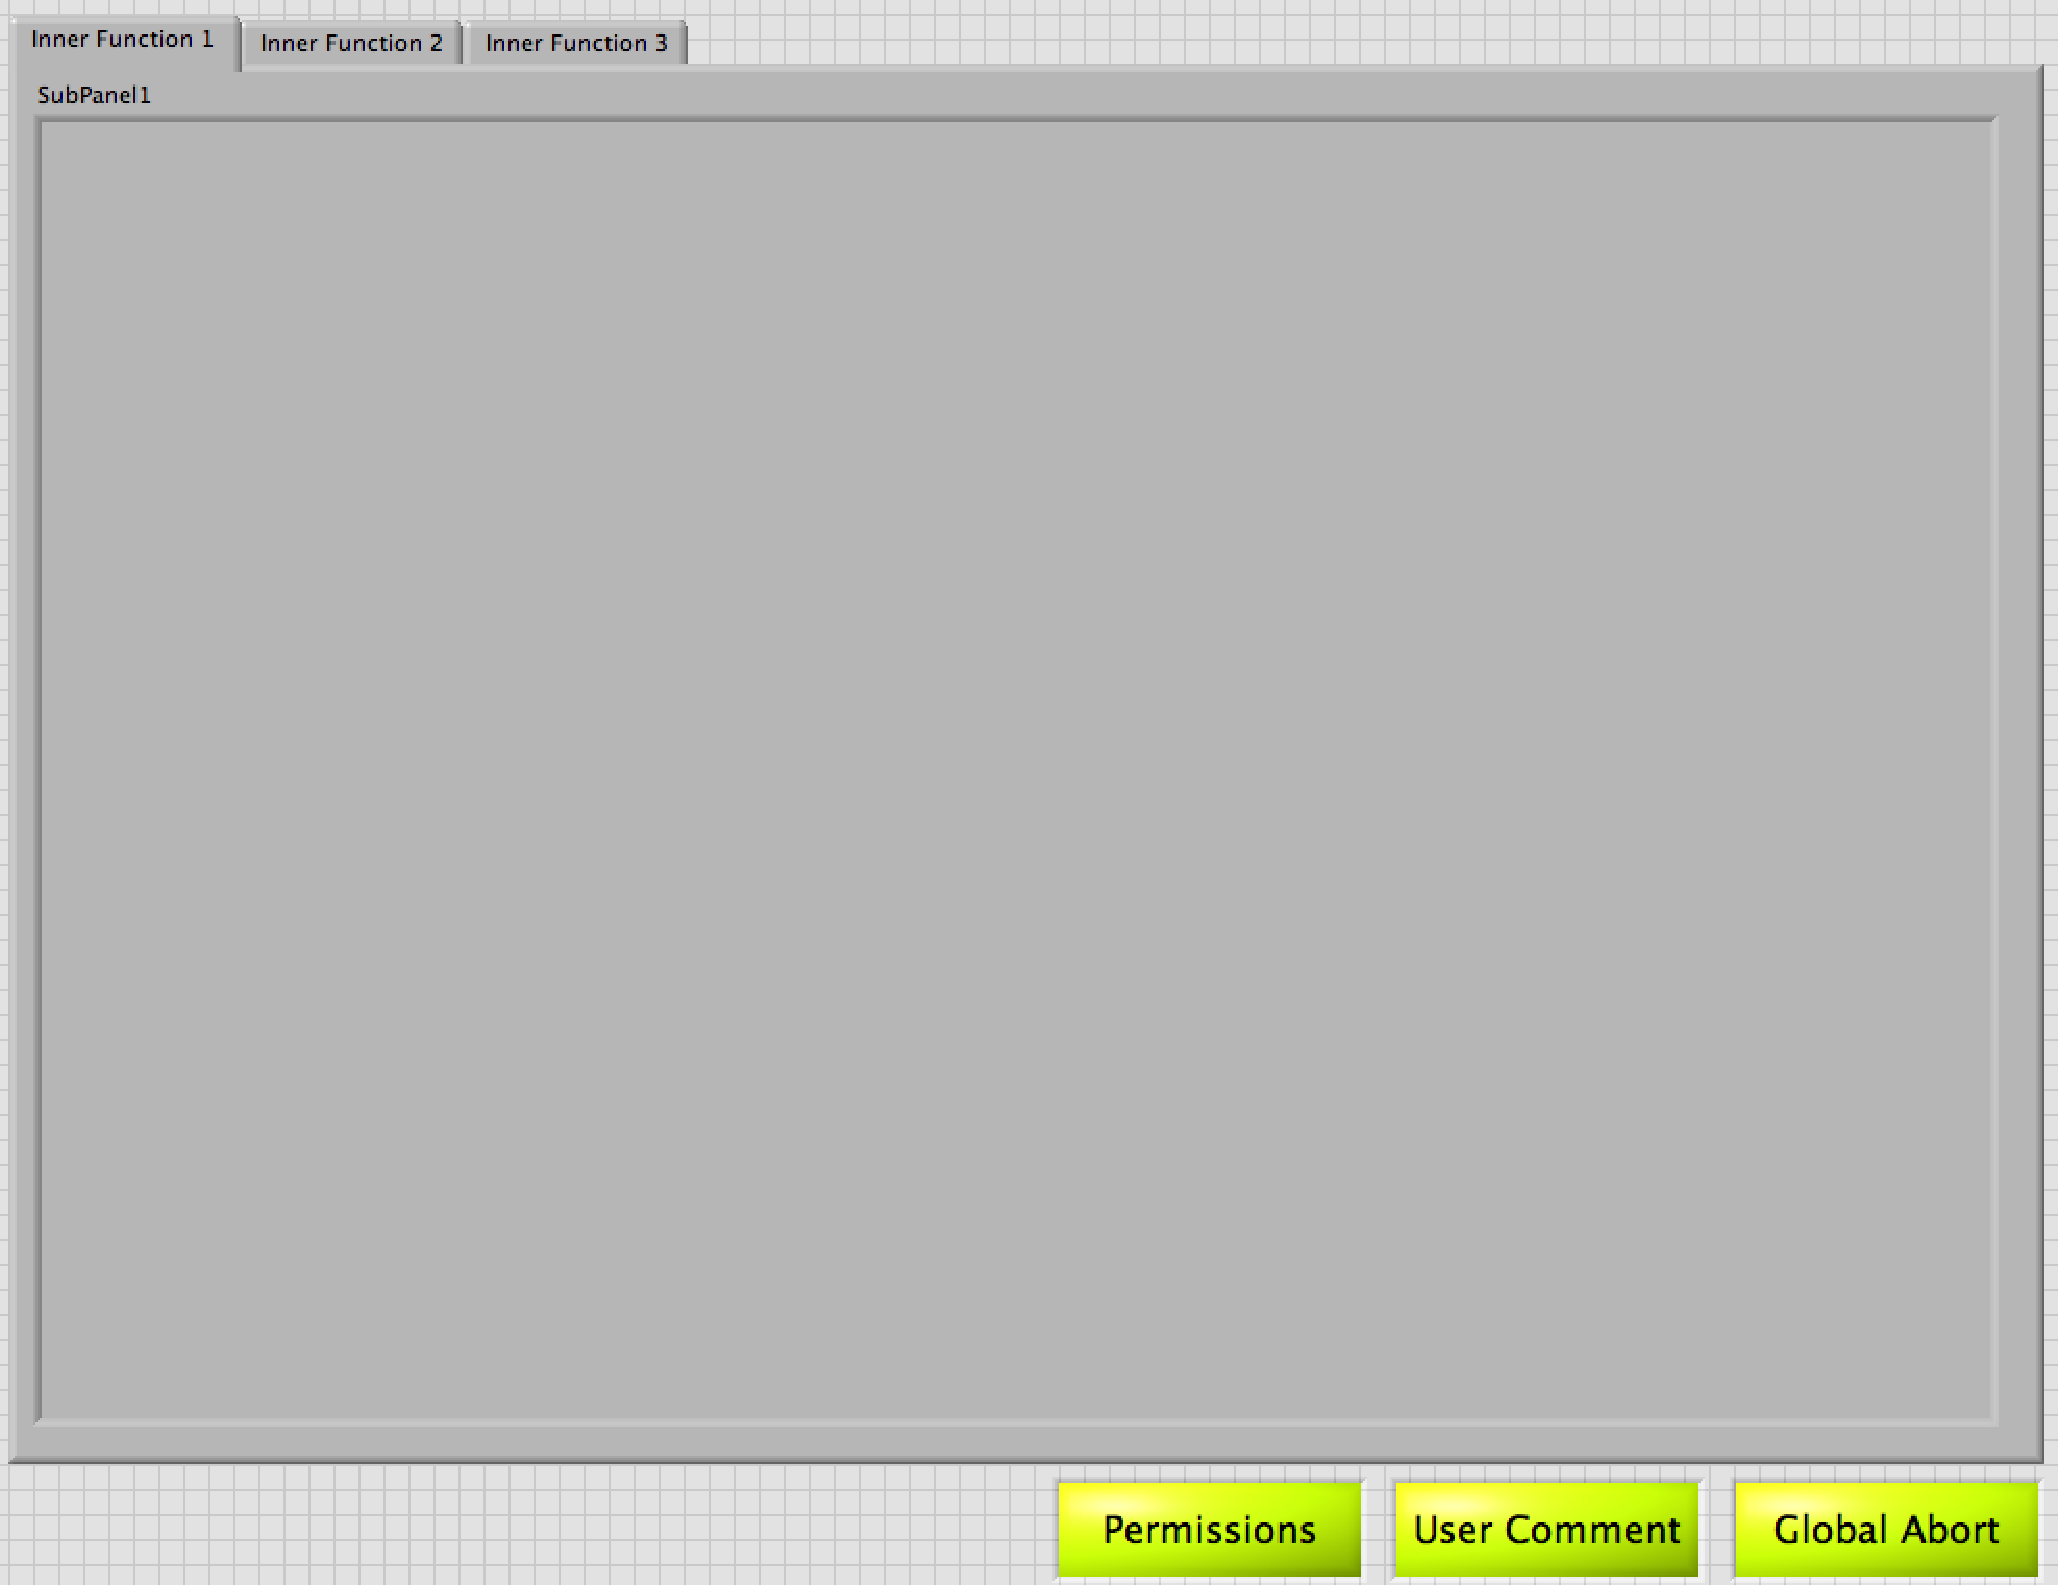
\includegraphics[height=3in]{Figures/MainVIContainer.eps}
\caption{The front panel of the main VI container. If multiple VIs are called and run simultaneously, their front panels are projected into the main container to allow for a simple control for the user but also allows maximum flexibility in VI execution.}\label{Fig:VIContainer}
\end{figure}

In this case, the controls that are common to all VIs, in the bottom box of Figure \ref{Fig:VITemplate}, are collected and included only once. Because the front panels of all VIs are to be projected into a single container, the front panel sizes of all VIs should be of a standard size otherwise the container would not simplify much. The container itself  is simply a set of sub-panels that can each hold a single VI. The maximum number of VIs needed can be written then if fewer are required, the main program can simply hide unused sub-panels. 

To my knowledge, the only problem with this approach is that sub-panels can not be collected into an array. As such, the maximum number of contents is not a particularly dynamic element. I need to look into this more to see if this can be arbitrary. 

\subsubsection{Configure Files}
Instead of using default variables in Labview, the default configuration for each sub program will be stored in a configuration file. This ensures that operational hardware configurations are decoupled from any software upgrades or changes. Additionally, it makes it always possible to return the software to a known pre-set operational state and makes it more difficult for users to unknowingly modify the hardware's initial state. The current plan is to allow the user with the proper credentials (see Section \ref{Sec:Password} for more details) to write new configure files from Labview directly to save a current state. That state file can be version controlled via Git to track its changes over time. An example of a simplified configure file is given in Figure \ref{Fig:ConfigureFile}. 

\begin{figure}[!h]\centering
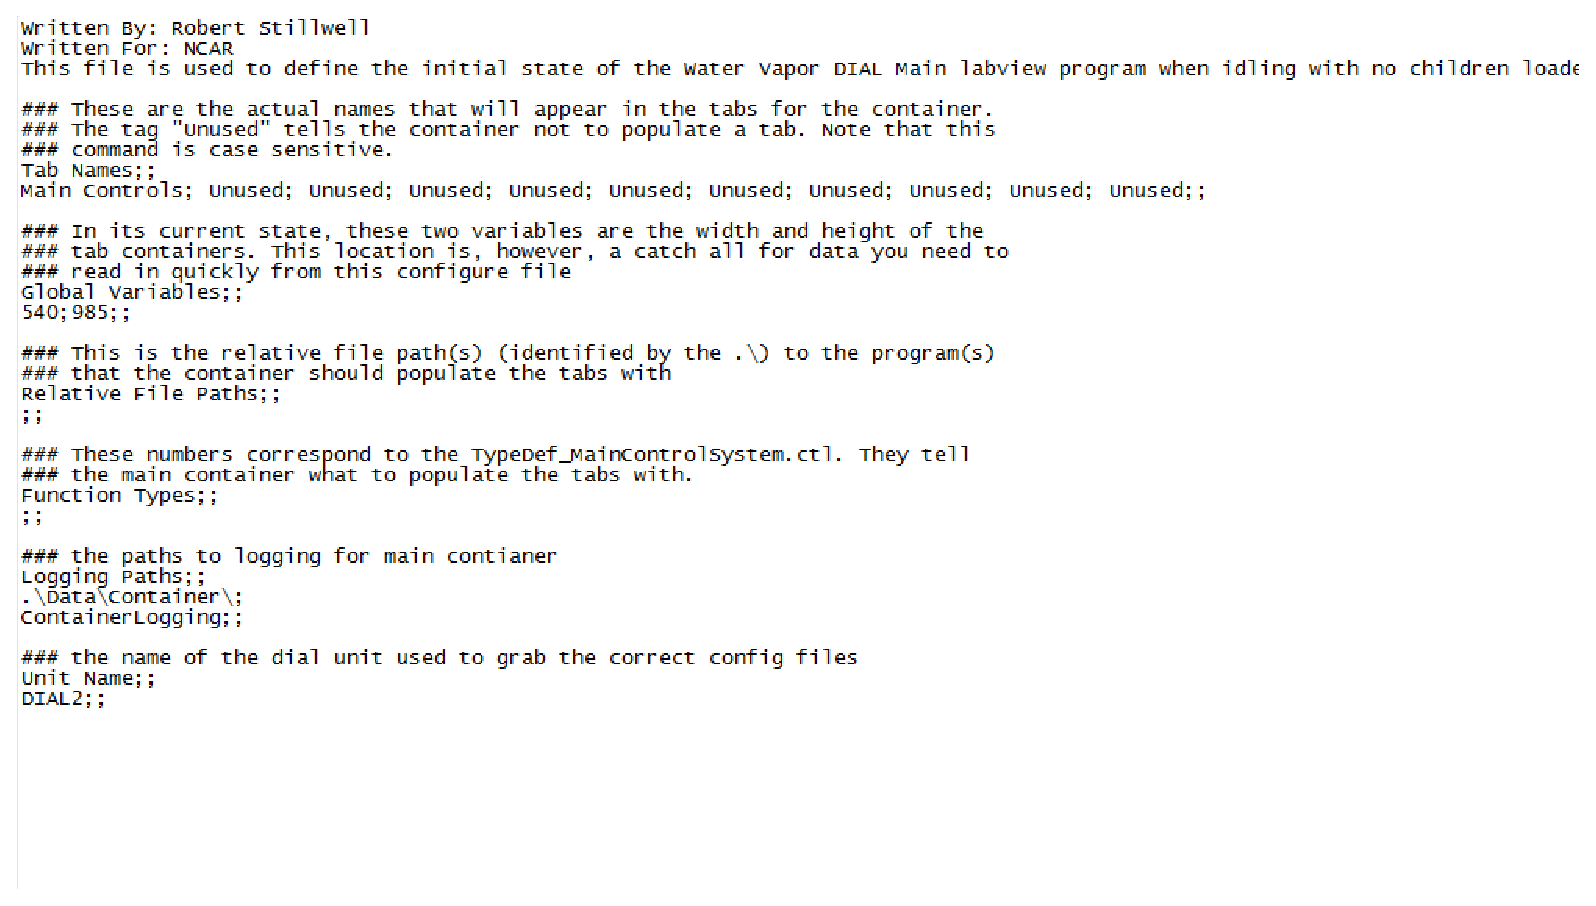
\includegraphics[height=3in]{Figures/ConfigureFileExample.eps}
\caption{An example of the structure of a configure file. Variables are identified by a single name followed by two semi-colons. The next line has the required values delimitated by a single semi-colon with the end of line denoted by a double semi-colon.}\label{Fig:ConfigureFile}
\end{figure}

\subsubsection{Log Files}

Log files are to be kept to help track the status of WV DIAL and to help debug any anomalous states. The logs to be kept are:

\begin{enumerate}
\item{Operations Log: Describes when the system starts and stops and any errors observed}
\item{System Status Log: Tracks the user defined changes from the configure status}
\item{User Comment Log: Allows for users to make comments about the operation of the system. An example would be if the system is found in an anomalous state and the debugging information used to recover or the reasons for a system status change. }
\end{enumerate}

\subsubsection{Type Definitions}

One of the most annoying features of labview occurs when trying to modify the contents of a complicated structure. For example, if you initially make a cluster to define the state of a single laser and wish to add a piece to that structure, labview will show each connected wire as broken throughout the entire program. To solve this, labview allows the user to define structure types and to link the controls on all panels directly to that definition. This allows the user to make a change in a single place and have all variables referenced to that place change at the same time. 

This type definition will be used for all controls. It requires an extra step to make the definition then load it into the program much like defining a global variable but it makes updating and maintaining the code cleaner. One example of this is the control used to define the main loop cases from Section \ref{Sec:BPDesign}.

\subsection{Sub-Functions and Calling}

All of the individual controls are collected into a single container to run more complicated tasks. For example, the main operation of WV DIAL at full capability would require simultaneous control of the MCS, weather station, laser locking and housekeeping, and visualization. The proposed labview code would simply run the 6 individual controls responsible for each of these tasks and store them in a single container. 

If a single VI fails, the other sub-functions are not affected by it. Its data would be missing from the global data however. For example, if the weather station communication failed, that data would be missing but it is not completely critical to have at all times. When its service could be restored, its data stream would be restored. 

\subsection{Main Function and Calling}

The concept of the main function is simply as a separate function to organize all the possible software possibilities of WV DIAL and to serve as a watchdog function. The current plan is to have each sub level report a status to the level above it. The idea is to make each level report that it is okay. If not, the level above it can fire off a warning signal to a user that the software is not running properly. I imagine a status email being sent periodically when the status is abnormal for example. 


\newpage 
